% !TEX root = SegwayDoku.tex

% in der ersten Zeile steht ein "magischer Kommentar". Dadurch weiß das Editierprogramm immer, welche Datei die Hauptdatei ist.

% die folgenden Zeilen werden benötigt, damit der richtige Author in der Fußzeile der Seite auftaucht.
\newpage
\renewcommand{\autoren}{Severin Schendel}

\section{Kippwinkelerkennung}

Das Ziel war es, die Kippwinkelerkennung des Roboters um die y-Achse zu verbessern, da bei der Ausgangsversion die Erkennung zu langsam und ungenau war. Es wurde weiterhin der Beschleunigungs- und Gyrosensor MPU6050 verwendet.

\subsection{Inbetriebnahme des MPU6050}
Der MPU6050 wurde an einem Arduino Mega2560 in Betrieb genommen und anschließend wurde das Programm auf den verwendenten Mikrocontroller des Roboters übersetzt.
\subsubsection{Auslesen der Rohwerte des Sensors}
Die Beschleunigungs- und Drehraterohwerte werden mit folgenden Befehlen ausgelesen.
\begin{lstlisting}[language=C++, caption=Auslesen der Sensorwerte, label={lst:Sensorwerte}]
#include "I2Cdev.h"
#include "MPU6050.h"
int16_t accY, accX, accZ, gyroY, gyroZ, gyroX;
MPU6050 mpu;

void loop() 
{
  accX = mpu.getAccelerationX();
  accY = mpu.getAccelerationY();
  accZ = mpu.getAccelerationZ(); 
  
  gyroX = mpu.getRotationX();
  gyroY = mpu.getRotationY();
  gyroZ = mpu.getRotationZ();
}
\end{lstlisting}

\subsubsection{Berechnung des Neigungswinkels \(\beta\)}
Der Neigungswinkel \(\beta\) wird einmal über den Beschleunigungssensor mit der arctan2 Funktion berechnet und einmal über das Gyroskop indem es die Winkelgeschwindigkeit über die Zeit integriert. Der Vorteil der arctan2 Funktion ist, dass sie zwei reelle Zahlen als Argument benutzt und somit den Funktionswert in einem Wertebereich von 360\(\degree\) ausgibt.

\begin{lstlisting}[language=C++, caption=Berechnen der Winkel, label={lst:Winkel}]
..
..
#define sampleTime  0.005

ISR(TIMER1_COMPA_vect)
 	{   
 	gyroRate = map(gyroZ, -32768, 32767, -250, 250);
	Acc_Pitch = atan2(accZ, accX)*RAD_TO_DEG;
	Gyro_Pitch =(float)gyroRate*sampleTime; 
	}
\end{lstlisting}

\subsection{Sensordatenfusion}
Um eine brauchbare Qualität der Winkel zu erhalten werden die beiden berechneten Winkel mit einem Filter fusioniert.

Folgende zwei Möglichkeiten wurden untersucht:
\begin{itemize}
	\item Komplementär Filter
	\item Kalman Filter
\end{itemize} 

\subsubsection{Komplementär Filter}
Die Idee hinter dem Komplementär Filter ist, dass man die kurzzeitig hohe Genauigkeit des Gyroskop(abdriften) mit der langfristigen Genauigkeit des Beschleunigungssensors(kein driften) kombiniert.

\begin{figure}[h]  % [h] bedeutet, dass das Bild genau an dieser Stelle im Text erscheint
% mit width=... wird die Größe des Bildes in Prozent der Seitenbreite eingestellt
\centering\includegraphics[width=0.7\textwidth]{images/komplementärfilter.eps}
% caption ist die Bildunterschrift, taucht auch im Abbildungsverzeichnis auf
\caption{Schematischer Aufbau eines Komplementärfilter \newline (Quelle: eigene Darstellung)}
\label{Komplementärfilter} % über das label kann man aus dem Text auf das Bild verweisen
\end{figure}

\textbf{Formel Komplementär Filter}

Formel zur Berechnung des neuen Winkels. 

\(\tau\) = Zeitkonstante des Filters.
\begin{flalign}
    % durch das & Zeichen werden alle Gleichungen an diesem Punkt ausgerichtet
	Angle  & = \alpha * (Angle + GyroPitch*dt)+ (1-\alpha)*AccPitch
	\label{eq:Komplementär Filter} \\
	\alpha &= \frac{\tau}{\tau*dt}
	\label{eq:Alpha }
\end{flalign}

  
\subsubsection{Kalman Filter}
Der Ansatz des Kalman Filter ist, dass man aus gemessenen fehlerbehafteten Werten eine möglichst genaue Schätzung bekommt über den tatsächlichen Zustand. 
\begin{figure}[h]  % [h] bedeutet, dass das Bild genau an dieser Stelle im Text erscheint
% mit width=... wird die Größe des Bildes in Prozent der Seitenbreite eingestellt
\centering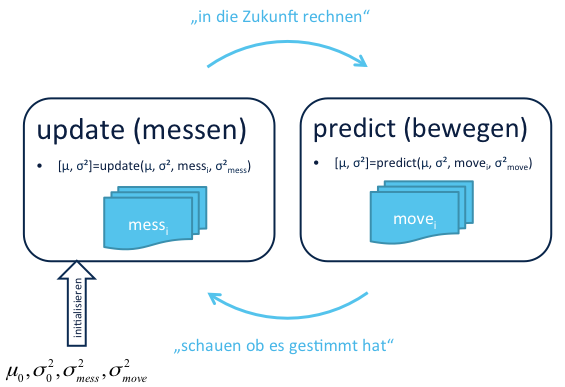
\includegraphics[width=0.7\textwidth]{images/Kalman-Filterstruktur.png}
% caption ist die Bildunterschrift, taucht auch im Abbildungsverzeichnis auf
\caption{Kalman Filter Ablauf \newline (Quelle: http://www.cbcity.de/))}
\label{Sturktur Kalman Filter} % über das label kann man aus dem Text auf das Bild verweisen
\end{figure}

\textbf{Umsetzung des Kalman Filters}

Der Kalman Filter wurde mit einem vorhandenen Skript implementiert.

\subsection{Bewertung}
Bei der Auswahl des geeigneten Filters wurde auf verschieden Kriterien geachtet. Diese werden in nachfolgender Tabelle aufgeführt.


\begin{tabular}{lll}
& Komplementär Filter & Kalman Filter\\
Winkel-Änderungsverhalten & +++& ++ \\
Störsicherheit & +++ &++++\\
Implementierung &++++ &+\\	
&&\\	
\end{tabular}

Aufgrund des besseren Winkel-Änderungsverhaltens haben wir uns für den Komplementär Filter entschieden. Jedoch hat der Filter für einen präzisen Winkel alleine nicht ausgereicht, sodass der Winkel nochmal über 10 aufeinanderfolgende Werte gemittelt wird.







\newpage
